\chapter{An\'alisis y Dise\~no de la Soluci\'on}

\section{Metodolog\'ia de Trabajo y Gobernanza MLOps}

Para garantizar que los hallazgos cient\'ificos de esta investigaci\'on sean verificables y reproducibles, se adopt\'o una metodolog\'ia de ingenier\'ia de software y operaciones de aprendizaje autom\'atico (\textit{MLOps}) basada en contratos de datos inmutables y trazabilidad criptogr\'afica. En proyectos de visi\'on artificial complejos, los errores silenciosos de preparaci\'on —tales como la fuga de datos (\textit{data leakage}), la reordenaci\'on no determinista de lotes o la sustituci\'on inadvertida de im\'agenes corruptas— invalidan cualquier conclusi\'on te\'orica.

La arquitectura de datos de DoctorMaiz desacopla tres conceptos fundamentales:
\begin{enumerate}
\item \textbf{Identidad (\texttt{sample\_id}):} Cada fotograf\'ia del corpus posee un identificador \'unico e inmutable calculado como $\text{SHA-256}(\text{ruta l\'ogica normalizada en UTF-8})$. Esto previene que el orden de lectura en el disco o la asignaci\'on estoc\'astica de hilos (\textit{workers}) altere la identidad de la muestra.
\item \textbf{Integridad (\texttt{sha256}):} Se calcula el hash criptogr\'afico SHA-256 directo sobre los bytes crudos del archivo de imagen. Esto permite auditar de forma autom\'atica si un archivo sufri\'o alteraciones, corrupci\'on o recomposici\'on entre distintas versiones de entrenamiento.
\item \textbf{Procedencia y Grupo (\texttt{source\_id} y \texttt{effective\_group\_id}):} Cada registro conserva el v\'inculo con su repositorio de origen, c\'amara y sesi\'on de captura, permitiendo construir particiones estratificadas por fuente sin filtrar datos asociados.
\end{enumerate}

Todos los conjuntos de entrenamiento, validaci\'on y prueba quedaron sellados mediante manifiestos contractuales (\texttt{manifest.lock.json}), garantizando cero solapamientos de muestras cross-split.

\section{Clases Agron\'omicas Objetivo}

El sistema clasifica el estado de salud de la hoja de ma\'iz en nueve categor\'ias mutuamente excluyentes (Tabla~\ref{tab:taxonomia}), abarcando los principales pat\'ogenos f\'ungicos, virales, plagas insectiles y deficiencias nutricionales de impacto econ\'omico en Centroam\'erica.

\begin{table}[H]
\caption{Taxonom\'ia agron\'omica de las nueve clases integradas en DoctorMaiz}
\label{tab:taxonomia}
\centering
\small
\begin{singlespace}
\begin{tabularx}{\textwidth}{>{\raggedright\arraybackslash}p{3.0cm}>{\raggedright\arraybackslash}p{3.9cm}>{\raggedright\arraybackslash}X>{\raggedright\arraybackslash}p{4.2cm}}
\toprule
\textbf{Clase Agron\'omica} & \textbf{Agente Causal / Tipo} & \textbf{S\'intoma Primario} & \textbf{Riesgo / Impacto en Rendimiento} \\
\midrule
\textbf{Roya Com\'un} & \textit{Puccinia sorghi} (Hongo) & P\'ustulas pulverulentas casta\~no-rojizas en ambas caras. & P\'erdida del 15\% al 30\% en \'areas h\'umedas y altas. \\
\textbf{Tiz\'on Foliar (NCLB)} & \textit{Exserohilum turcicum} (Hongo) & Lesiones alargadas en forma de cigarro o huso (grises). & Necrosis masiva, p\'erdidas de hasta 50\% antes de floraci\'on. \\
\textbf{Mancha Gris (GLS)} & \textit{Cercospora zeae-maydis} (Hongo) & Manchas rectangulares delimitadas por venas secundarias. & Destrucci\'on del follaje superior, reducci\'on del grano hasta 40\%. \\
\textbf{Necrosis Letal (MLN)} & Complejo viral sin\'ergico (MCMV + Potyvirus) & Clorosis severa, moteado, necrosis marginal y secado total. & \textbf{P\'erdida del 100\% de la cosecha}; patolog\'ia de bioseguridad cr\'itica. \\
\textbf{Gusano Cogollero} & \textit{Spodoptera frugiperda} (Plaga/Insecto) & Perforaciones irregulares y excrementos en el cogollo. & Destrucci\'on meristem\'atica; ca\'ida de rendimiento del 20\% al 60\%. \\
\textbf{Deficiencia de Nitr\'ogeno} & Desbalance nutricional abi\'otico & Clorosis en ``V'' invertida desde la punta hacia la base. & Reducci\'on de porte, espigas peque\~nas y bajo llenado. \\
\textbf{Deficiencia de F\'osforo} & Desbalance nutricional abi\'otico & Coloraci\'on p\'urpura o rojiza en bordes de hojas j\'ovenes. & Retraso radicular y esterilidad parcial de la mazorca. \\
\textbf{Deficiencia de Potasio} & Desbalance nutricional abi\'otico & Clorosis y necrosis marginal desde el \'apice foliar. & Acame o volcamiento del tallo y grano liviano. \\
\textbf{Planta Sana (Healthy)} & Control agron\'omico & L\'amina foliar verde homog\'enea sin lesiones ni plagas. & Crecimiento \'optimo seg\'un potencial gen\'etico del cultivar. \\
\bottomrule
\end{tabularx}
\end{singlespace}
\end{table}

\begin{figure}[H]
\centering
\begin{minipage}[b]{0.31\linewidth}
\centering
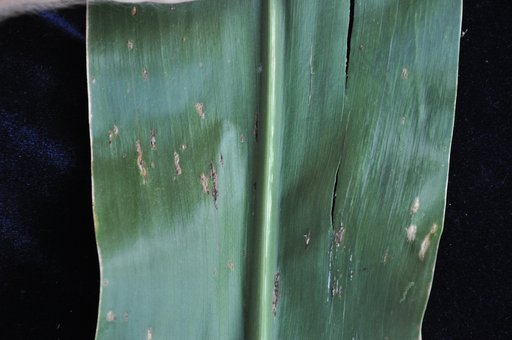
\includegraphics[width=\linewidth]{images/dataset-classes/common_rust.jpg}
\caption*{a) Roya Com\'un}
\end{minipage}
\hfill
\begin{minipage}[b]{0.31\linewidth}
\centering
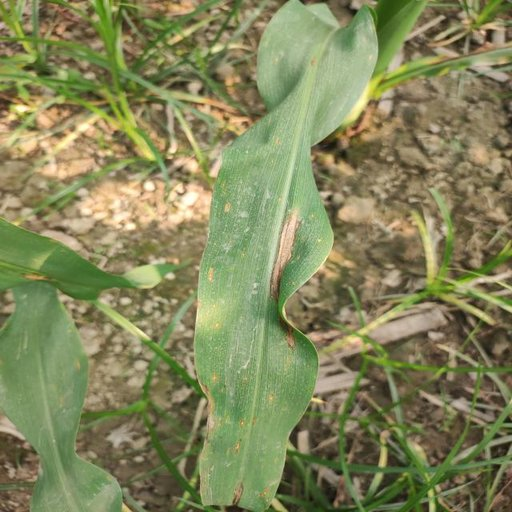
\includegraphics[width=\linewidth]{images/dataset-classes/northern_corn_leaf_blight.jpg}
\caption*{b) Tiz\'on Foliar}
\end{minipage}
\hfill
\begin{minipage}[b]{0.31\linewidth}
\centering
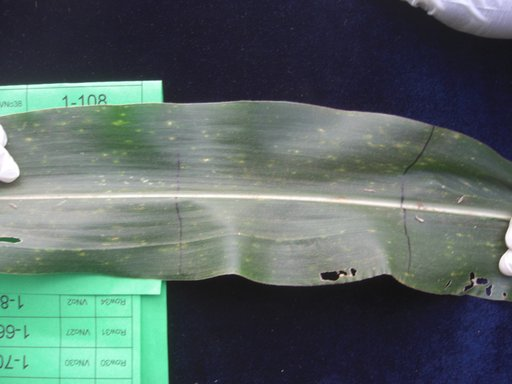
\includegraphics[width=\linewidth]{images/dataset-classes/gray_leaf_spot.jpg}
\caption*{c) Mancha Gris}
\end{minipage}

\vspace{0.3cm}
\begin{minipage}[b]{0.31\linewidth}
\centering
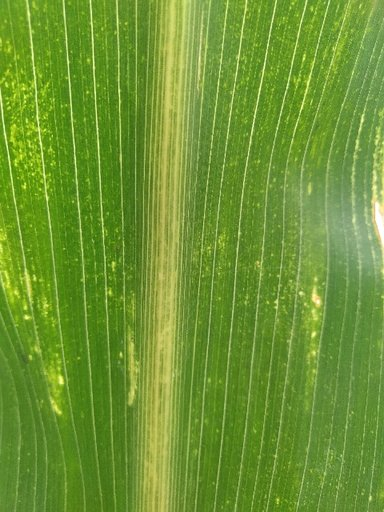
\includegraphics[width=\linewidth]{images/dataset-classes/lethal_necrosis.jpg}
\caption*{d) Necrosis Letal}
\end{minipage}
\hfill
\begin{minipage}[b]{0.31\linewidth}
\centering
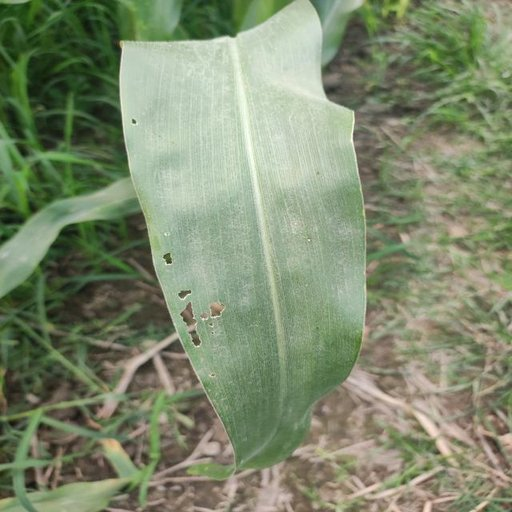
\includegraphics[width=\linewidth]{images/dataset-classes/fall_armyworm.jpg}
\caption*{e) Gusano Cogollero}
\end{minipage}
\hfill
\begin{minipage}[b]{0.31\linewidth}
\centering
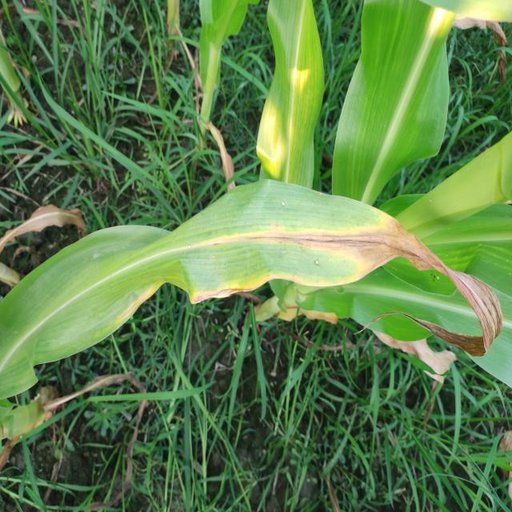
\includegraphics[width=\linewidth]{images/dataset-classes/nitrogen_deficiency.jpg}
\caption*{f) Deficiencia N}
\end{minipage}

\vspace{0.3cm}
\begin{minipage}[b]{0.31\linewidth}
\centering
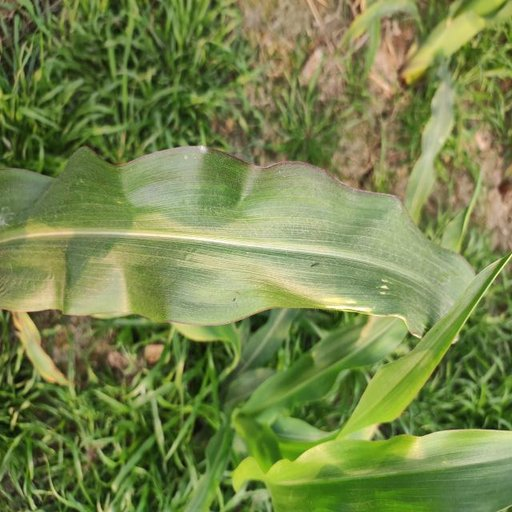
\includegraphics[width=\linewidth]{images/dataset-classes/phosphorus_deficiency.jpg}
\caption*{g) Deficiencia P}
\end{minipage}
\hfill
\begin{minipage}[b]{0.31\linewidth}
\centering
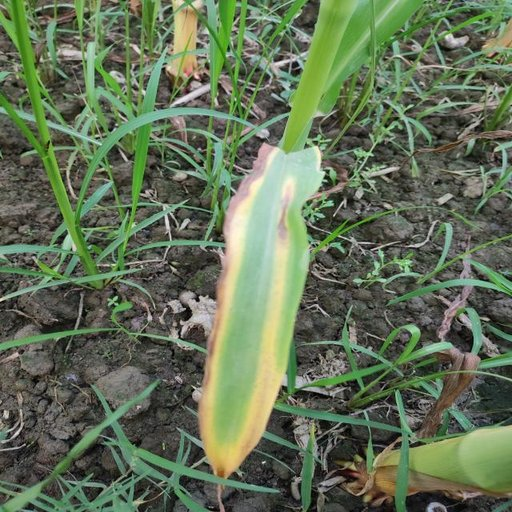
\includegraphics[width=\linewidth]{images/dataset-classes/potassium_deficiency.jpg}
\caption*{h) Deficiencia K}
\end{minipage}
\hfill
\begin{minipage}[b]{0.31\linewidth}
\centering
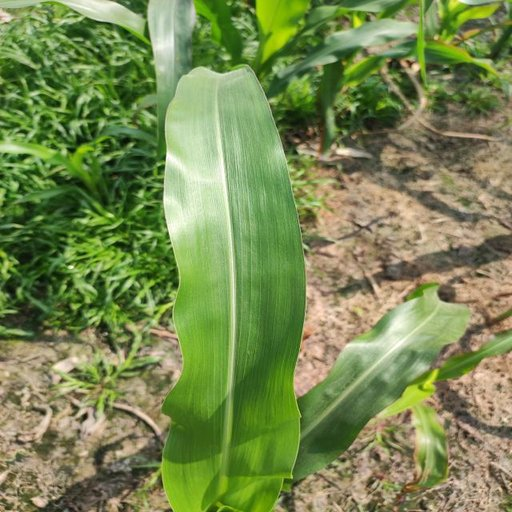
\includegraphics[width=\linewidth]{images/dataset-classes/healthy.jpg}
\caption*{i) Planta Sana}
\end{minipage}
\caption{Cat\'alogo fotogr\'afico de las nueve clases agron\'omicas presentes en el corpus.}
\label{fig:clases_mosaico}
\end{figure}

\section{Recopilaci\'on, Depuraci\'on y Auditor\'ia de Datos}

El corpus final se conform\'o mediante la integraci\'on de \textbf{33~429 im\'agenes elegibles} provenientes de 11 fuentes internacionales consolidadas (Tabla~\ref{tab:fuentes_dataset}). Para resolver el cuello de botella identificado en la primera fase del proyecto —donde la deficiencia de potasio colapsaba a un $F_1$ de 0.49 debido a la escasez extrema de muestras—, se incorporaron cuatro repositorios dirigidos a deficiencias minerales.

\begin{table}[H]
\caption{Fuentes de datos recopiladas y distribuci\'on de muestras}
\label{tab:fuentes_dataset}
\centering
\small
\begin{singlespace}
\begin{tabularx}{\textwidth}{p{6.6cm}ccp{3.6cm}}
\toprule
\textbf{Identificador de Fuente (\texttt{source\_id})} & \textbf{Muestras} & \textbf{Entorno} & \textbf{Patolog\'ias Principales Aportadas} \\
\midrule
\texttt{maize-beans-tomatoes-africa} & 12~136 & Mixto & 4 clases. \\
\texttt{maize-diseases} & 6~989 & Campo Real & 3 clases. \\
\texttt{multicrop-disease-maiz} & 5~816 & Campo Real & 3 clases, incluida necrosis letal (MLN). \\
\texttt{corn-leaf-roboflow} & 2~919 & Mixto & 6 clases. \\
\texttt{cropdg-unified-multidomain} & 2~562 & Mixto & 3 clases. \\
\texttt{maize-in-field-dataset} & 852 & Campo Real & 3 clases. \\
\texttt{maize-2-roboflow} & 846 & Mixto & 3 clases. \\
\texttt{corn-leaf-diseases-}\allowbreak\texttt{classification-roboflow} & 480 & Mixto & 1 clase (\texttt{gray\_leaf\_spot}). \\
\texttt{maize-nutrient-deficiency} & 340 & Mixto & 4 clases. \\
\texttt{maize-leaf-roboflow} & 331 & Mixto & 1 clase. \\
\texttt{maize-deficiency-}\allowbreak\texttt{scanner-roboflow} & 158 & Campo Real & 3 clases de deficiencia. \\
\midrule
\textbf{Total Elegible Auditado} & \textbf{33~429} & — & \textbf{9 clases agron\'omicas} \\
\bottomrule
\end{tabularx}
\end{singlespace}
\end{table}

\subsection{Data Profiling y An\'alisis Exploratorio de Datos (EDA)}
El an\'alisis exploratorio evidenci\'o tres retos estructurales:
\begin{itemize}
\item \textbf{Desbalance intr\'inseco:} La clase sana concentra cerca de 8~700 im\'agenes y el tiz\'on foliar cerca de 6~800, mientras que la deficiencia de potasio cuenta con 621 ejemplares (desbalance de 14.1:1 en el corpus vigente, frente a 32.9:1 antes de la ampliaci\'on).
\item \textbf{Heterogeneidad de resoluci\'on y c\'amaras:} Las resoluciones van desde sensores r\'usticos de $256\times256$ p\'ixeles hasta capturas semiprofesionales de $4000\times3000$ p\'ixeles (Figura~\ref{fig:eda_distribuciones}).
\item \textbf{Asociaci\'on espuria fuente-clase:} La asociaci\'on estad\'istica entre la procedencia y la etiqueta arroj\'o una \textbf{V de Cram\'er de 0.5030}, indicando que ciertas fuentes p\'ublicas aportan exclusivamente una sola patolog\'ia, lo que puede favorecer que las redes utilicen señales del entorno además de la lesión foliar. Esta relación es descriptiva y no establece una causa.
\end{itemize}

\begin{figure}[H]
\centering
\begin{minipage}[b]{0.48\linewidth}
\centering
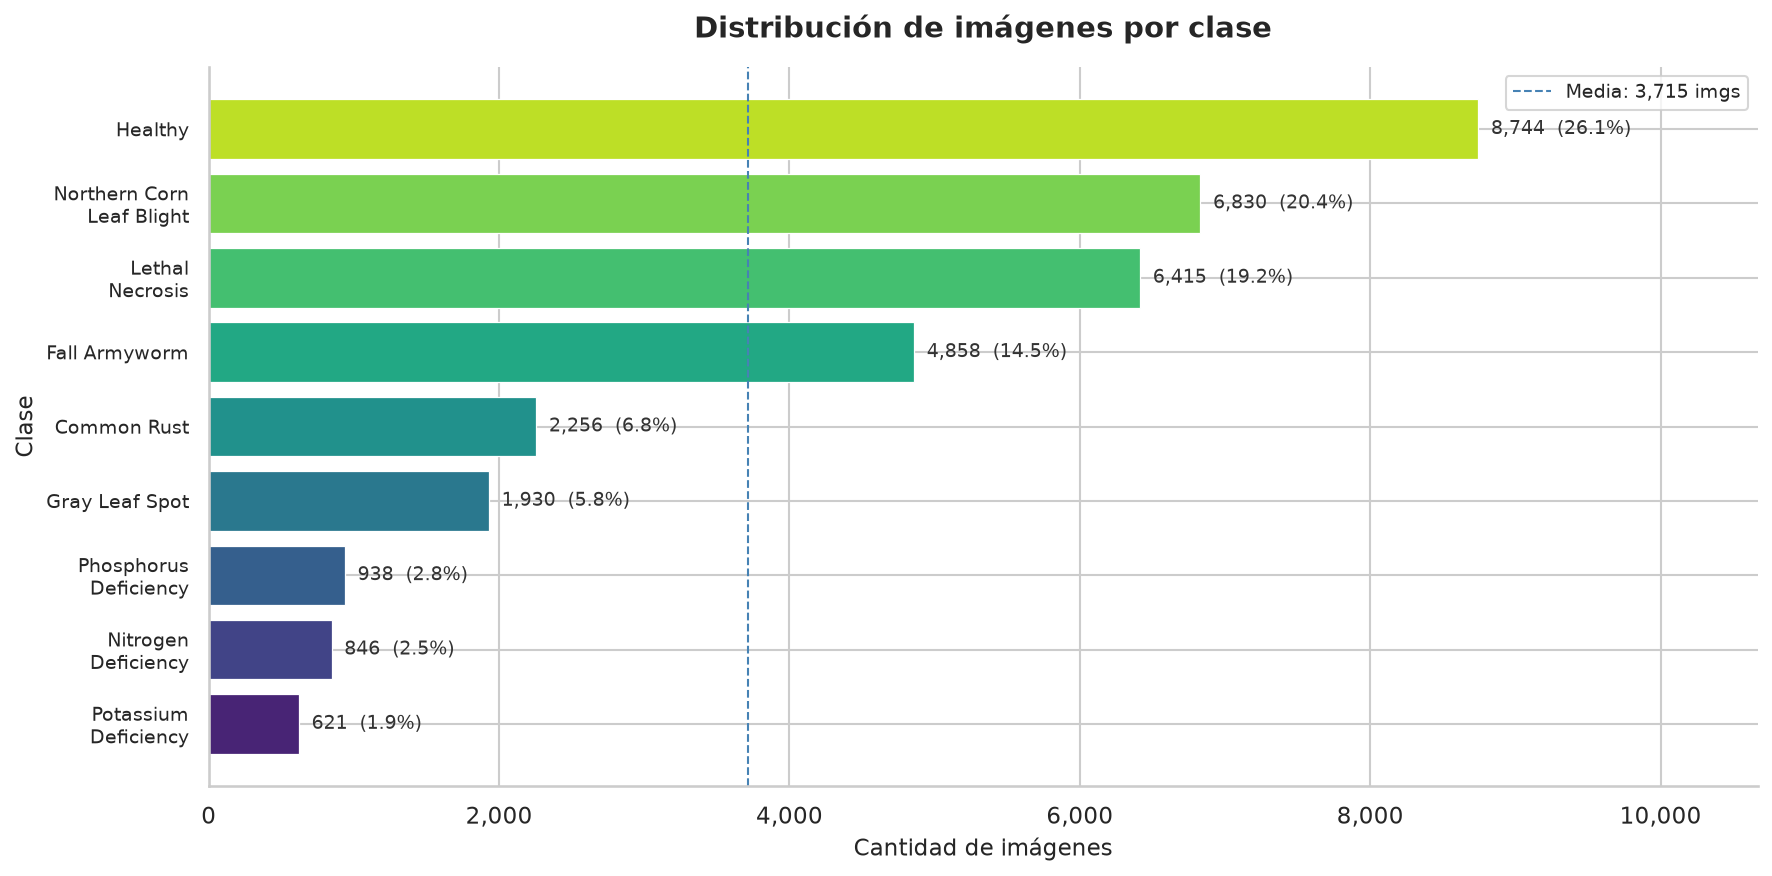
\includegraphics[width=\linewidth]{images/eda/eda_01_distribucion_clases.png}
\caption{Distribuci\'on de muestras por clase.}
\label{fig:eda_clases}
\end{minipage}
\hfill
\begin{minipage}[b]{0.48\linewidth}
\centering
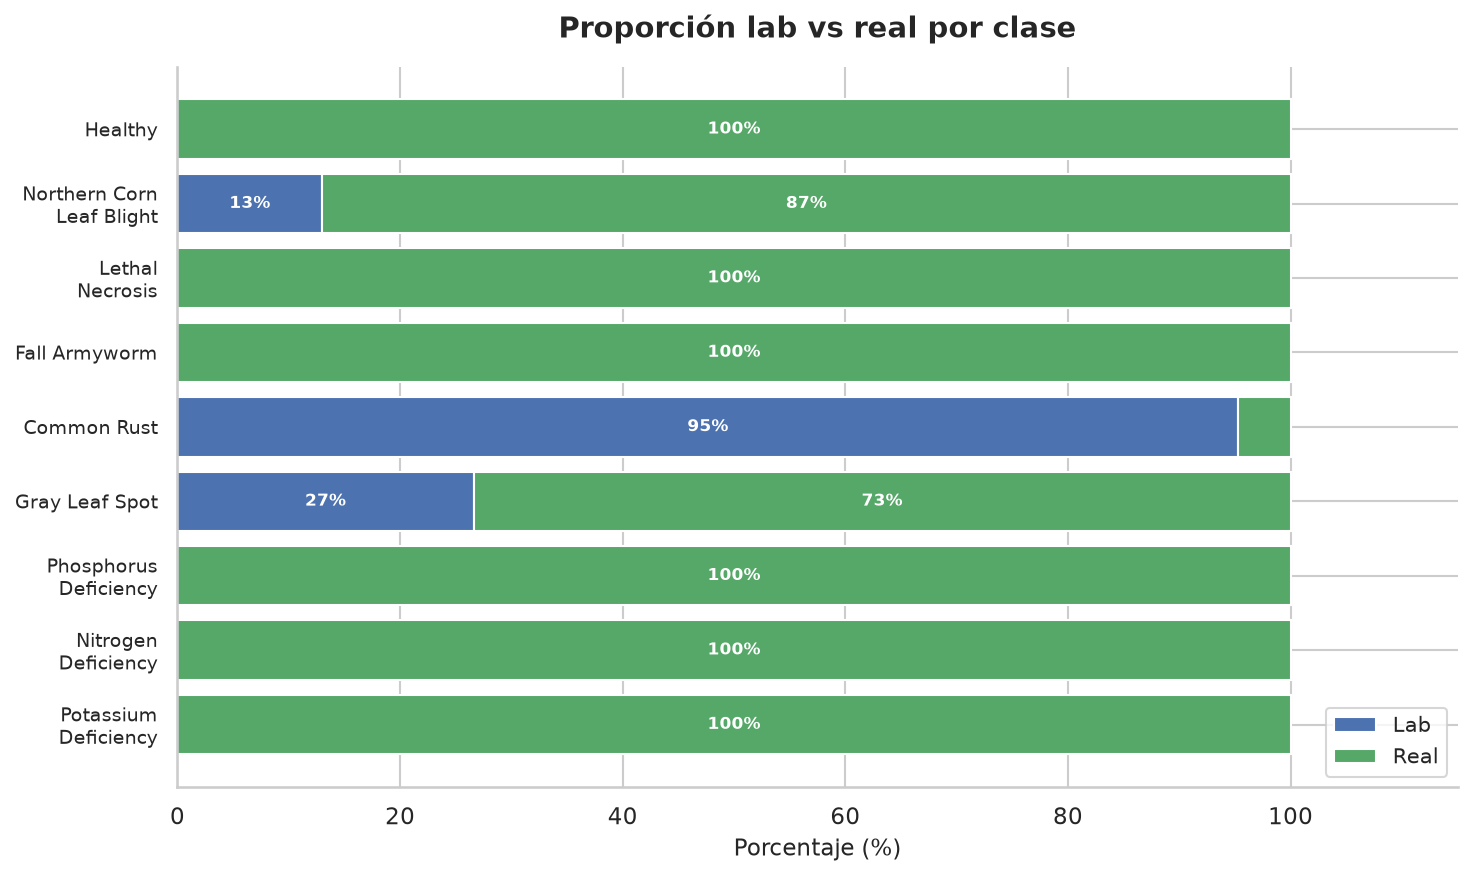
\includegraphics[width=\linewidth]{images/eda/eda_02_lab_vs_real.png}
\caption{Proporci\'on Laboratorio vs. Campo Real.}
\label{fig:eda_lab_real}
\end{minipage}
\caption{An\'alisis exploratorio de distribuci\'on y balance ambiental del corpus.}
\label{fig:eda_distribuciones}
\end{figure}

\begin{figure}[H]
\centering
\begin{minipage}[b]{0.48\linewidth}
\centering
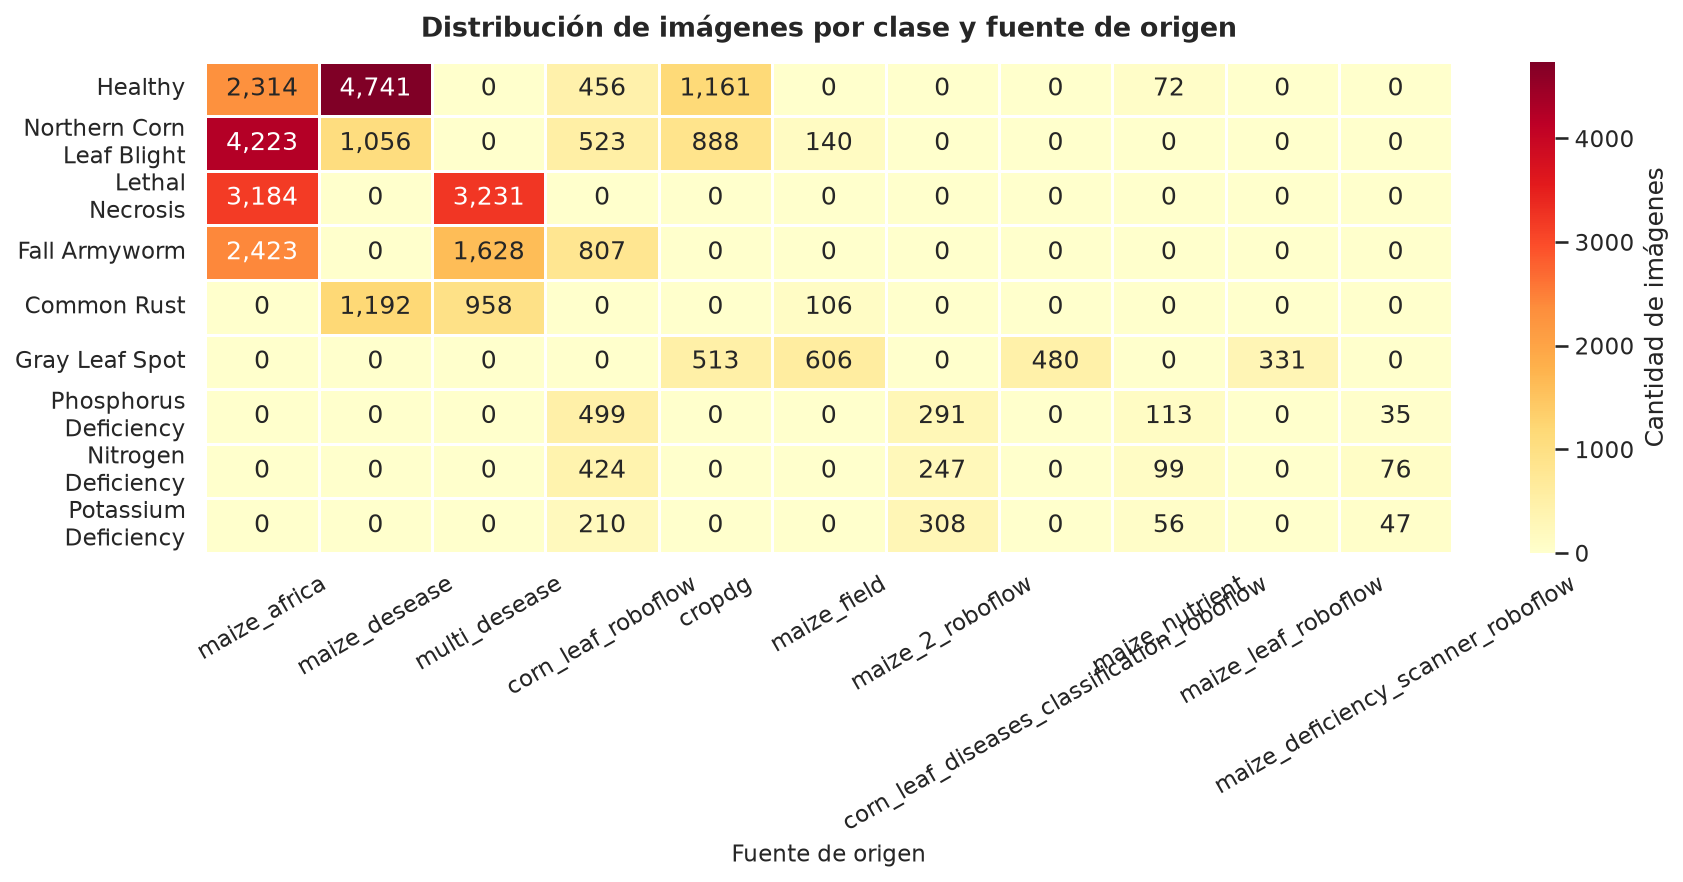
\includegraphics[width=\linewidth]{images/eda/eda_02b_heatmap_fuente_clase.png}
\caption{Matriz de contingencia fuente vs. patolog\'ia.}
\label{fig:eda_heatmap}
\end{minipage}
\hfill
\begin{minipage}[b]{0.48\linewidth}
\centering
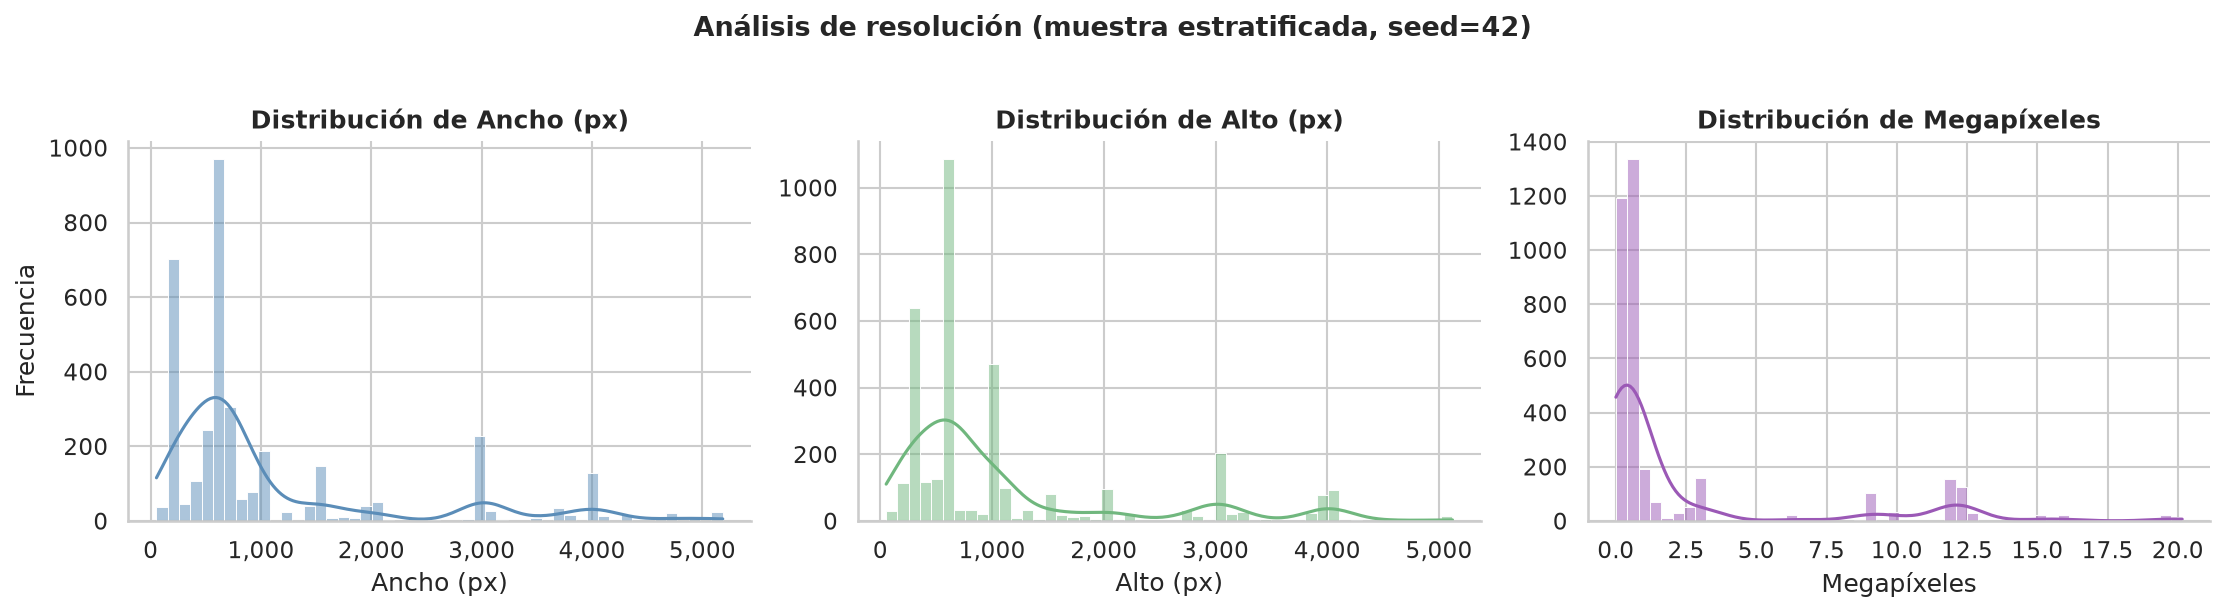
\includegraphics[width=\linewidth]{images/eda/eda_03_resoluciones.png}
\caption{Distribuci\'on de resoluciones espaciales.}
\label{fig:eda_resoluciones}
\end{minipage}
\caption{Concentraci\'on de procedencia y heterogeneidad geom\'etrica en las im\'agenes.}
\end{figure}

\subsection{Auditor\'ia Criptogr\'afica de P\'ixeles}
Para descartar que la precisi\'on reportada se inflara por duplicados id\'enticos en entrenamiento y prueba, se ejecut\'o la auditor\'ia \texttt{PIXEL\_DUPLICATE\_AUDIT}. Se calcularon hashes SHA-256 directos sobre el contenido decodificado en memoria. Se descubrieron \'unicamente cuatro grupos de im\'agenes (ocho archivos en total) con etiquetas contradictorias entre repositorios, los cuales fueron purgados de inmediato. Las \textbf{33~429 muestras finales no presentan un solo duplicado id\'entico cross-split}.

La partici\'on de desarrollo oficial (\texttt{seed\_42}) qued\'o estructurada en un reparto estratificado 70/15/15:
\begin{itemize}
\item \textbf{Entrenamiento:} 23~400 im\'agenes.
\item \textbf{Validaci\'on:} 5~014 im\'agenes.
\item \textbf{Prueba independiente (Test retenido):} 5~015 im\'agenes.
\end{itemize}

\noindent\textbf{Limitaci\'on de la partici\'on de desarrollo.} La partici\'on \texttt{seed\_42} es estratificada por \texttt{label + environment} y mezcla las fuentes conocidas entre entrenamiento, validaci\'on y prueba. Esta configuraci\'on es adecuada para desarrollo \textit{in-distribution}, pero no demuestra generalizaci\'on a una c\'amara, parcela o repositorio nuevo. Adem\'as, la materializaci\'on se gener\'o con \texttt{deduplicate\_perceptual=false}, por lo que la posible fuga por im\'agenes casi duplicadas no fue medida en este trabajo. La evaluaci\'on agrupada por fuente y el estudio \textit{leave-one-source-out} se presentan en el cap\'itulo de resultados.

\section{Arquitecturas y B\'usqueda de Hiperpar\'ametros}

\subsection{Familias Convolucionales Seleccionadas}
Se seleccionaron tres redes convolucionales modernas de alta eficiencia, representativas de diversas hip\'otesis inductivas:
\begin{enumerate}
\item \textbf{EfficientNet-Lite0 (Modelo m\'ovil desplegado):} Variante dise\~nada espec\'ificamente para inferencia m\'ovil y cuantizaci\'on. Elimina las activaciones no lineales complejas (\textit{swish}) sustituy\'endolas por ReLU6, y suprime los bloques de atenci\'on \textit{Squeeze-and-Excitation} (SE) \cite{hu2018} para mantener compatibilidad plena con aceleradores de enteros (3.38 millones de par\'ametros) \cite{tan2019}.
\item \textbf{EfficientNet-B0 (Referencia de capacidad):} Arquitectura balanceada con escalado compuesto y bloques SE con atenci\'on por canal (4.02 millones de par\'ametros).
\item \textbf{ShuffleNet-V2-x1.0 (Eficiencia extrema):} Basada en divisi\'on de canales (\textit{Channel Split}) y barajado (\textit{Channel Shuffle}) para maximizar el flujo de informaci\'on minimizando los accesos a memoria DRAM (1.26 millones de par\'ametros) \cite{ma2018}.
\end{enumerate}

\subsection{Espacio de B\'usqueda y Poda Temprana}
La optimizaci\'on de hiperpar\'ametros se formul\'o mediante un estudio bayesiano en \textbf{Optuna} \cite{optuna2019} con el estimador de \'arbol de Parzen multivariado (TPE). La funci\'on objetivo maximiz\'o el Macro $F_1$ sobre el conjunto de validaci\'on oficial. Para no desperdiciar horas de GPU en configuraciones no prometedoras, se incorpor\'o el algoritmo \textbf{MedianPruner}: a partir de la \'epoca 8 (periodo de calentamiento), si el Macro $F_1$ de un ensayo se sit\'ua por debajo de la mediana hist\'orica de los ensayos precedentes, el entrenamiento se detiene autom\'aticamente (\textit{PRUNED}).

El espacio de exploraci\'on abarc\'o siete par\'ametros cr\'iticos (Tabla~\ref{tab:hpo_espacio}).

\begin{table}[H]
\caption{Espacio de b\'usqueda de hiperpar\'ametros explorado con Optuna}
\label{tab:hpo_espacio}
\centering
\small
\begin{singlespace}
\begin{tabularx}{\textwidth}{lp{4.2cm}X}
\toprule
\textbf{Hiperpar\'ametro} & \textbf{Rango / Opciones} & \textbf{Fundamento Ingenieril} \\
\midrule
\texttt{learning\_rate} & Log-uniforme: $[10^{-5}, 3\times10^{-3}]$ & Control de convergencia en optimizador AdamW. \\
\texttt{batch\_size} & Categ\'orico: $\{16, 32, 64\}$ & Estabilidad del gradiente estoc\'astico y saturaci\'on de GPU. \\
\texttt{weight\_decay} & Log-uniforme: $[10^{-6}, 10^{-2}]$ & Regularizaci\'on $L_2$ para mitigar memorizaci\'on de fondos. \\
\texttt{class\_weights} & $\{\text{none}, \text{inv}, \text{sqrt\_inv}\}$ & Ponderaci\'on de p\'erdida para compensar desbalance de clases. \\
\texttt{label\_smoothing} & Uniforme: $[0.0, 0.15]$ & Calibraci\'on probabil\'istica y prevenci\'on de sobreconfianza. \\
\texttt{warmup\_epochs} & Entero: $[1, 5]$ & Calentamiento lineal para proteger pesos preentrenados. \\
\texttt{clahe} & Fijo en \texttt{False} & Ecualizaci\'on adaptativa excluida de la b\'usqueda; se evalu\'o aparte. \\
\bottomrule
\end{tabularx}
\end{singlespace}
\end{table}

\subsection{Ensamble Multimodelo por Soft Voting}
Para mitigar el riesgo de diagn\'osticos err\'oneos causados por las zonas ciegas de una sola arquitectura, se implement\'o un ensamble heterog\'eneo por votaci\'on suave. El ensamble calcula el vector de probabilidades promedio:
\begin{equation}
P_{\text{ens}}(y = c \mid x) = \frac{1}{M} \sum_{m=1}^{M} P_m(y = c \mid x)
\end{equation}
donde $M=3$ corresponde a las tres redes entrenadas independientemente y $c \in \{1, \dots, 9\}$. La decisi\'on final se obtiene por consenso m\'aximo: $\hat{y} = \arg\max_c P_{\text{ens}}(y = c \mid x)$.

\section{Despliegue en Dispositivo M\'ovil}

\subsection{Cuantizaci\'on a Enteros de 8 Bits (Int8)}
Para permitir que \texttt{EfficientNet-Lite0} opere en tel\'efonos sin unidad de procesamiento neuronal (\textit{NPU}), se realiz\'o una cuantizaci\'on posterior al entrenamiento (\textit{Post-Training Quantization}, PTQ) \cite{jacob2018} hacia enteros de 8 bits, exportando el modelo mediante litert-torch. El esquema es simétrico (punto cero $Z = 0$) y dinámico: las escalas de activación se calculan en tiempo de ejecución, por lo que no requiere un conjunto de calibración. En el backbone, cada canal de salida $c$ tiene su propia escala $S_c$, que mapea los pesos en coma flotante $W_{f,c,i}$ a enteros con signo:
\begin{equation}
S_c = \frac{\max_i \lvert W_{f,c,i} \rvert}{127}, \qquad q_{c,i} = \operatorname{clip}\!\left(\left\lfloor \frac{W_{f,c,i}}{S_c} \right\rceil,\; -127,\; 127\right)
\end{equation}
La capa lineal final usa una \'unica escala por tensor, porque el kernel de TFLite para \texttt{FULLY\_CONNECTED} dinámico aplica una sola escala. Con escalas por canal, los logits de esa capa quedan multiplicados por una constante distinta por clase sin que el runtime lo señale. Cuantizar todas las capas por tensor, en cambio, degrada las convoluciones \textit{depthwise} de EfficientNet, cuyos pesos tienen rangos muy distintos entre canales; por ello el backbone se cuantiza por canal. La operaci\'on permite que las multiplicaciones de matrices de convoluci\'on se resuelvan con instrucciones vectoriales enteras en la CPU m\'ovil. El consumo energ\'etico no fue medido en este trabajo.

\subsection{Detector de Anomal\'ias Fuera de Distribuci\'on (OOD)}
Las redes neuronales pueden emitir clasificaciones con alta confianza cuando reciben im\'agenes que no pertenecen a ninguna de sus clases, por ejemplo suelo, calzado o malezas, porque la confianza softmax solo mide la elecci\'on entre las etiquetas conocidas \cite{lee2018}. Para detectar este caso, DoctorMaiz extrae el vector de activaci\'on de la capa previa a la clasificaci\'on ($d = 1~280$ dimensiones), reduce su dimensionalidad mediante PCA a 186 componentes que retienen el 99\,\% de la varianza y eval\'ua la \textbf{Distancia Relativa de Mahalanobis (RMD)} \cite{ren2021}. La distancia resta un modelo de fondo global para no penalizar caracter\'isticas gen\'ericas de cualquier fotograf\'ia:
El vector se normaliza a norma L2 unitaria antes de proyectarlo \cite{mahalanobispp2025}. La puntuaci\'on es
\begin{equation}
\text{RMD}(z) = D_M\!\left(z \,\middle|\, \mu_{c^*}, \Sigma\right) - D_M\!\left(z \,\middle|\, \mu_0, \Sigma_0\right)
\end{equation}
donde $\mu_{c^*}$ es el centroide de la clase m\'as cercana, $\Sigma$ es la covarianza agrupada entre clases y $\mu_0$, $\Sigma_0$ describen una gaussiana de fondo sobre todo el conjunto de entrenamiento. Ambas covarianzas se regularizan con un t\'ermino ridge proporcional a su traza antes de invertirlas.

El umbral se calibra sobre el conjunto de validaci\'on, no visto durante el entrenamiento, como el percentil 95 de la puntuaci\'on de cada hoja v\'alida. El umbral de la aplicaci\'on instalada est\'a pendiente de regeneraci\'on: el archivo de estad\'isticas OOD que empaqueta la aplicaci\'on no tiene un run de origen registrado. El modelo instalado corresponde al run \texttt{20260812\_221429} (SHA-256 del \texttt{.tflite} verificado), pero su archivo \texttt{ood\_stats.json} no existe en la exportaci\'on de ese run. El valor se obtendr\'a al ejecutar \texttt{compute\_ood\_stats.py} sobre dicho checkpoint. Las pruebas sint\'eticas (pantallas negras, ruido aleatorio) superaron valores de 300 y las fotograf\'ias reales de campo quedaron por debajo del umbral. Si la puntuaci\'on supera el umbral, la aplicaci\'on muestra la advertencia \textbf{«Imagen no reconocida»} y no emite diagn\'ostico.

\subsection{Mitigaci\'on en la Interfaz: Marco Gu\'ia y Severidad}
Como se demostrar\'a en el cap\'itulo de resultados, el software no puede eliminar por completo los atajos de fondo de los repositorios p\'ublicos. Por ello, la soluci\'on integr\'o dos innovaciones directas en la aplicaci\'on:
\begin{enumerate}
\item \textbf{C\'amara con marco gu\'ia foliar y recorte autom\'atico:} La interfaz superpone una silueta ergon\'omica de la hoja con la instrucci\'on expl\'icita: \textit{«Ac\'erquese a 20--30 cm y llene el marco»}. La aplicaci\'on recorta la imagen capturada a la regi\'on delimitada por el marco gu\'ia antes de pasar la matriz al modelo, de modo que el \'area enviada corresponde a la hoja y no al entorno completo.
\item \textbf{Gu\'ia de severidad en lenguaje campesino:} Dado que los modelos de clasificaci\'on no pueden predecir el porcentaje de \'area foliar comprometida, la app despliega debajo de la etiqueta una escala visual de tres niveles (baja, moderada, cr\'itica) basada en manuales homologados del CIMMYT e Iowa State, descrita en t\'erminos coloquiales y recomendando bioinsumos accesibles en el agroservicio local.
\end{enumerate}

\section{Segmentaci\'on de Hojas: dos usos y resultados}

El proyecto utiliz\'o la segmentaci\'on foliar en dos l\'ineas distintas, con evidencia y estado diferentes. Ninguna de ellas forma parte de la predicci\'on de la aplicaci\'on instalada, que recorta geom\'etricamente la imagen con el marco gu\'ia.

	extbf{Primer uso: presegmentaci\'on y entrenamiento sobre corpus enmascarado.} El pipeline del clasificador incluye un m\'odulo de segmentaci\'on (	exttt{src/segmentation}) que genera un corpus con m\'ascaras de hoja. Se entren\'o un modelo sobre ese corpus (run 	exttt{20260907\_163546}, EfficientNet-Lite0, sobre el split 	exttt{seed\_42\_segmented}). Su Macro $F_1$ en prueba fue de 	extbf{0.7191} y su accuracy de 0.8903, frente a 0.9480 del baseline de imagen completa vigente. Esta comparaci\'on no es pareada: el conjunto de prueba segmentado no comparte ninguna imagen con el conjunto de prueba original (0 de 5~015 rutas coinciden). El perfil de m\'ascara usado para generar el corpus no est\'a registrado en el resumen del run, por lo que el resultado no permite atribuir la ca\'ida a un perfil concreto. El proyecto clasifica este uso como experimental y no como preprocesamiento general.

	extbf{Segundo uso: segmentador de instancias para aislar la hoja.} En un repositorio independiente se entren\'o un segmentador YOLO (	exttt{yolo26n-seg}, Ultralytics 8.4.104) para seleccionar la hoja principal. La configuraci\'on D-01 cambi\'o un solo hiperpar\'ametro (	exttt{mosaic=0}) sobre la configuraci\'on base de semilla 42 y se evalu\'o \'unicamente sobre validaci\'on. Obtuvo 	extit{Mask mAP50-95} de 0.94404 y 	extit{Mask recall} de 0.94309. Sobre 150 hojas enfermas de validaci\'on, el quality gate marc\'o 150 m\'ascaras como 	exttt{reliable}, con IoU medio de 0.98122 y Dice medio de 0.99046. Estos resultados son de una sola semilla y no incluyen evaluaci\'on sobre el conjunto de prueba ni sobre el piloto de fuente externa, que siguen sin ejecutarse.

La implicaci\'on para el dise\'no es que una m\'ascara puede eliminar se\~nal \'util del fondo. Por ello el proyecto no aplica segmentaci\'on de forma universal, y la comparaci\'on formal entre imagen completa y segmentada sigue pendiente.


\section{Sincronizaci\'on y Contribuci\'on al Dataset Colaborativo}

La aplicaci\'on funciona sin servidor. Esta secci\'on describe el dise\~no de la sincronizaci\'on opcional, implementado en el repositorio de la API. Su comportamiento descrito aqu\'i proviene del c\'odigo y de la especificaci\'on de dise\~no; las pruebas de integraci\'on previstas en esa especificaci\'on no se han ejecutado en este trabajo.

El dise\~no contempla dos tipos de registro que la aplicaci\'on env\'ia cuando hay conexi\'on y una cuenta registrada: correcciones de diagn\'ostico y aportes fotogr\'aficos al dataset colaborativo. Ambos se almacenan en MySQL 8.4 y no se incluye telemetr\'ia de escaneos ni coordenadas GPS del historial.

Los dos endpoints de escritura son \texttt{POST /corrections} y \texttt{POST /dataset-contributions}. La especificaci\'on define que ambos sean idempotentes por el par \texttt{(user\_id, client\_id)}: un reenv\'io con el mismo identificador debe devolver el registro existente en lugar de duplicarlo. Tambi\'en define un l\'imite de 30 solicitudes por minuto por usuario autenticado. El env\'io de imagen se valida como archivo de imagen antes de guardarse. Estas tres propiedades son de dise\~no; su verificaci\'on queda pendiente.

El env\'io previsto incluye la fotograf\'ia, la etiqueta elegida, una nota opcional y la fecha del escaneo. No incluye nombre, tel\'efono, correo ni coordenadas GPS. La aplicaci\'on no elimina los metadatos EXIF de la fotograf\'ia antes de enviarla, por lo que este punto queda como pendiente de tratamiento.

Sin cuenta registrada, la aplicaci\'on conserva los aportes en el tel\'efono y no los env\'ia. La cola de sincronizaci\'on reintenta cuando hay conexi\'on.

\subsection{Modelo relacional de la base de datos del servidor}

El servidor almacena cinco tablas en MySQL 8.4, definidas en la migración inicial de Alembic. La Figura~\ref{fig:er_api} muestra sus relaciones. La única dependencia entre tablas es que cada registro de usuario agrupa sus tokens de sesión y sus aportes, y la tabla de versiones de la aplicación no se relaciona con las demás.

\begin{figure}[H]
\centering
\begin{tikzpicture}[
  ent/.style={draw=blue!55!black, fill=blue!4, rounded corners=2pt, align=left, font=\scriptsize, inner sep=4pt, text width=4.2cm},
  rel/.style={-{Latex[length=2.2mm]}, line width=0.8pt, draw=gray!70}
]
\node[ent] (users) {\textbf{users}\\[1pt]
  id \emph{(PK)}\\ name, email \emph{(único)}\\ password\_hash, created\_at};
\node[ent, below=1.1cm of users, xshift=-5.6cm] (rt) {\textbf{refresh\_tokens}\\[1pt]
  id \emph{(PK)}\\ user\_id \emph{(FK)}\\ token\_hash \emph{(único)}, expires\_at, revoked\_at, created\_at};
\node[ent, below=1.1cm of users, xshift=0cm] (corr) {\textbf{corrections}\\[1pt]
  id \emph{(PK)}\\ user\_id \emph{(FK)}, client\_id\\ scan\_id, observed\_label, note, status\\ created\_at, received\_at\\ \emph{único:} (user\_id, client\_id)};
\node[ent, below=1.1cm of users, xshift=5.6cm] (dc) {\textbf{dataset\_contributions}\\[1pt]
  id \emph{(PK)}\\ user\_id \emph{(FK)}, client\_id\\ image\_path, label, note, status\\ created\_at, received\_at\\ \emph{único:} (user\_id, client\_id)};
\node[ent, below=5.2cm of users, xshift=0cm] (ar) {\textbf{app\_releases}\\[1pt]
  id \emph{(PK)}\\ platform, version\_code, version\_name\\ min\_supported\_version\_code\\ download\_url, release\_notes\\ published\_at, is\_active};
\draw[rel] (users.south west) -- ++(0,-0.4) -| (rt.north);
\draw[rel] (users.south) -- (corr.north);
\draw[rel] (users.south east) -- ++(0,-0.4) -| (dc.north);
\end{tikzpicture}
\caption{Modelo relacional del servidor. Las flechas van de \texttt{users} a las tablas que referencian su \texttt{id}. \texttt{app\_releases} no tiene relaciones.}
\label{fig:er_api}
\end{figure}

\subsection{Flujo de sincronizaci\'on desde la aplicaci\'on}

La Figura~\ref{fig:secuencia_sync} describe el recorrido de un aporte desde que el productor lo guarda hasta que el servidor lo confirma. El guardado es local e inmediato. La sincronizaci\'on se dispara al recuperar la red o por acci\'on del usuario, y antes de enviar comprueba en orden tres condiciones: que existan registros pendientes, que haya conexi\'on y que haya una sesi\'on. Si no hay pendientes, el proceso termina sin enviar nada. Si el servidor responde 401, la aplicaci\'on refresca el token una sola vez y reintenta. Un registro solo se marca como sincronizado tras la confirmaci\'on del servidor; si el env\'io falla, permanece pendiente para el siguiente intento.

\begin{figure}[H]
\centering
\begin{tikzpicture}[
  life/.style={draw=gray!60, line width=0.5pt, dashed},
  pt/.style={draw=blue!55!black, fill=blue!5, rounded corners=2pt, align=center, font=\scriptsize, minimum height=0.7cm, minimum width=2.4cm},
  msg/.style={-{Latex[length=2mm]}, line width=0.7pt},
  rmsg/.style={-{Latex[length=2mm]}, line width=0.7pt, dashed},
  self/.style={font=\tiny, align=left, draw=gray!50, fill=yellow!8, rounded corners=1pt, inner sep=2pt},
  lab/.style={font=\tiny, fill=white, inner sep=1pt}
]
\def\yp{0}
\node[pt] (P) at (0,0) {Productor};
\node[pt] (A) at (3.4,0) {App DoctorMaiz};
\node[pt] (D) at (6.8,0) {SQLite local};
\node[pt] (S) at (10.2,0) {Servidor (API)};
\draw[life] (P) -- (0,-9.2);
\draw[life] (A) -- (3.4,-9.2);
\draw[life] (D) -- (6.8,-9.2);
\draw[life] (S) -- (10.2,-9.2);

% 1 productor -> app : toma foto
\draw[msg] (0,-0.9) -- (3.4,-0.9) node[midway, lab, above] {1. Toma foto};
% 2 app -> sqlite : guarda pendiente
\draw[msg] (3.4,-1.6) -- (6.8,-1.6) node[midway, lab, above] {2. Guarda aporte pendiente};
% 3 confirmacion local
\draw[rmsg] (6.8,-2.1) -- (3.4,-2.1) node[midway, lab, above] {3. Confirmaci\'on local};

% 4 self: disparo
\draw[self] (3.4,-2.8) -- (3.4,-2.8);
\node[self, anchor=west] at (3.6,-2.9) {4. Disparo: cambio de red o bot\'on};

% 5 app -> sqlite : hay pendientes
\draw[msg] (3.4,-3.6) -- (6.8,-3.6) node[midway, lab, above] {5. \'Hay pendientes?};
% 6 respuesta
\draw[rmsg] (6.8,-4.1) -- (3.4,-4.1) node[midway, lab, above] {6. No: termina sin enviar};

% 6b alternative pending yes continues (self note)
\node[self, anchor=west] at (3.6,-4.8) {7. S\'i: comprueba red (NetInfo) y sesi\'on};

% 7 app -> servidor : POST sin token valido
\draw[msg] (3.4,-5.6) -- (10.2,-5.6) node[midway, lab, above] {8. POST aporte};
% 8 servidor -> app : 401
\draw[rmsg] (10.2,-6.1) -- (3.4,-6.1) node[midway, lab, above] {9. 401 si no hay sesi\'on};
% 9 refresh and retry
\draw[msg] (3.4,-6.6) -- (10.2,-6.6) node[midway, lab, above] {10. Refresca token y reintenta};
% 10 ack
\draw[rmsg] (10.2,-7.1) -- (3.4,-7.1) node[midway, lab, above] {11. 201 o 200 (confirmaci\'on)};
% 11 marca synced
\draw[msg] (3.4,-7.7) -- (6.8,-7.7) node[midway, lab, above] {12. Marca synced = true};

% failure branch note
\node[self, anchor=west] at (3.6,-8.4) {Si el env\'io falla: el registro queda pendiente};
\end{tikzpicture}
\caption{Flujo de sincronizaci\'on de un aporte, desde el guardado local hasta la confirmaci\'on del servidor. Si el env\'io falla, el registro permanece pendiente.}
\label{fig:secuencia_sync}
\end{figure}

\section{Arquitectura General del Sistema}

\subsection{Tecnolog\'ias por proyecto}

El sistema se compone de cuatro repositorios independientes. La Tabla~\ref{tab:tecnologias_c2} resume la pila tecnol\'ogica de cada uno, con las versiones fijadas en sus archivos de dependencias.

\begin{table}[H]
\caption{Tecnolog\'ias principales por proyecto}
\label{tab:tecnologias_c2}
\centering
\small
\begin{singlespace}
\begin{tabularx}{\textwidth}{>{\raggedright\arraybackslash}p{3.2cm}>{\raggedright\arraybackslash}p{4.2cm}X}
\toprule
\textbf{Proyecto} & \textbf{Funci\'on} & \textbf{Tecnolog\'ias} \\
\midrule
Pipeline del modelo & Entrenamiento, exportaci\'on y explicabilidad & PyTorch (\texttt{torch} 2.4 a 2.12), timm, Optuna, litert-torch y ONNX Runtime para exportaci\'on, Modal (GPU A10) para entrenamiento en la nube, SHAP y LIME. \\
Aplicaci\'on m\'ovil & Captura, inferencia local y sincronizaci\'on & Expo 57, React Native 0.86, TypeScript 6, \texttt{react-native-fast-tflite} 3 para inferencia, WatermelonDB 0.28 con SQLite local, NativeWind 4. \\
API de sincronizaci\'on & Versi\'on de la app y aportes al dataset colaborativo & FastAPI 0.115, SQLAlchemy 2.0, Alembic 1.13, MySQL 8.4 en Docker Compose, aiomysql, JWT y bcrypt para autenticaci\'on, slowapi para l\'imites de tasa. \\
Segmentador de hojas & Aislamiento de la l\'amina foliar (experimental) & Ultralytics 8.4.104 con modelo \texttt{yolo26n-seg}, PyTorch 2.2 a 2.12, Modal para entrenamiento, Pillow y NumPy. \\
\bottomrule
\end{tabularx}
\end{singlespace}
\end{table}

La separaci\'on en repositorios tiene una consecuencia pr\'actica: la aplicaci\'on no depende del entorno de entrenamiento. Solo consume un archivo \texttt{.tflite}, un \texttt{labels.json} y un \texttt{ood\_stats.json} empaquetados. La API y la aplicaci\'on se comunican por HTTP y MySQL solo existe en el servidor.


La Figura~\ref{fig:arquitectura_flujo} sintetiza la arquitectura de extremo a extremo que conecta la fase de experimentaci\'on con el despliegue m\'ovil y la extensi\'on institucional.

\begin{figure}[H]
\centering
\begin{tikzpicture}[
    node distance=0.7cm and 0.9cm,
    stage/.style={
        rectangle, rounded corners=4pt, draw=gray!50, line width=0.8pt,
        minimum width=2.9cm, minimum height=1.35cm, text width=2.7cm,
        align=center, font=\footnotesize, fill=gray!4
    },
    phase/.style={font=\scriptsize\bfseries\itshape, text=gray!60!black},
    arrow/.style={-{Latex[length=2.8mm]}, line width=1pt, draw=gray!60}
]
% --- Fila 1: entrenamiento ---
\node[phase] (lbl1) {Fase de entrenamiento y selecci\'on};
\node[stage, fill=blue!6, draw=blue!55!black, below=0.35cm of lbl1, xshift=-3.3cm] (datos)
  {\textbf{Fuentes p\'ublicas}\\[2pt]33~429 im\'agenes\\11 fuentes};
\node[stage, fill=blue!6, draw=blue!55!black, right=of datos] (pipe)
  {\textbf{Pipeline MLOps}\\[2pt]Deduplicaci\'on\\y contratos};
\node[stage, fill=blue!6, draw=blue!55!black, right=of pipe] (optuna)
  {\textbf{Optuna en GPU}\\[2pt]Poda temprana\\(25 intentos)};
\node[stage, fill=blue!6, draw=blue!55!black, right=of optuna] (lite0)
  {\textbf{EfficientNet-Lite0}\\[2pt]Configuraci\'on oficial\\[2pt]{\scriptsize run 20260921}};
\draw[arrow] (datos) -- (pipe);
\draw[arrow] (pipe) -- (optuna);
\draw[arrow] (optuna) -- (lite0);

% --- Fila 2: despliegue ---
\node[phase, below=1.3cm of datos, xshift=1.2cm] (lbl2) {Fase de despliegue m\'ovil};
\node[stage, fill=green!6, draw=green!45!black, below=0.35cm of lbl2, xshift=-3.3cm] (quant)
  {\textbf{Cuantizaci\'on Int8}\\[2pt]PTQ con litert-torch\\(3.56~MB)};
\node[stage, fill=green!6, draw=green!45!black, right=of quant] (app)
  {\textbf{App DoctorMaiz}\\[2pt]React Native\\y Fast-TFLite};
\node[stage, fill=green!6, draw=green!45!black, right=of app] (ood)
  {\textbf{Captura y OOD}\\[2pt]Marco gu\'ia y\\distancia RMD};
\node[stage, fill=green!6, draw=green!45!black, right=of ood] (off)
  {\textbf{Inferencia local}\\[2pt]CPU, sin conexi\'on\\(sincronizaci\'on opcional)};
\draw[arrow] (quant) -- (app);
\draw[arrow] (app) -- (ood);
\draw[arrow] (ood) -- (off);

% --- Conexi\'on entre filas ---
\draw[arrow, dashed] (lite0.south) |- ++(0,-0.55) -| (quant.north);
\end{tikzpicture}
\caption{Diagrama de flujo arquitect\'onico integral del sistema DoctorMaiz.}
\label{fig:arquitectura_flujo}
\end{figure}
